% !TeX encoding = UTF-8
% !TeX spellcheck = en_US

\chapter{Patterns in eMoflon::IBeX-GT}
\label{concept-and-implementation}
This chapter provides a short introduction to the architecture of the eMoflon::IBeX tool suite (Section~\ref{emoflon-ibex-architecture}) and describes the implementation of the graph transformation part in detail.
Section~\ref{ibex-patterns} explains the language features supported by the textual editor and the transformation into patterns for the pattern matcher.
The generated pattern networks are summarized in Section~\ref{pattern-networks}.

\section{eMoflon::IBeX Architecture}
\label{emoflon-ibex-architecture}
The eMoflon::IBeX tool suite is implemented as a set of plugins for the Eclipse IDE and supports both unidirectional and bidirectional model transformations.
Some functions such as code generation for meta-models and utilities for handling the interaction with the Eclipse framework are shared with eMoflon::SDM/TiE via eMoflon::Core.

Figure~\ref{fig:emoflon-ibex-components} gives an overview of the high-level architecture of eMoflon::IBeX.
The tool can be divided into the editor (green), its core functionality (blue) and the Democles adapter (orange). 
The GT and TGG rules are defined in textual editors based on the Xtext\footnote{\url{https://www.eclipse.org/Xtext/}} framework which provide features such as syntax highlighting, auto-completion, and validation.
Graphical visualizations are implemented with PlantUML.\footnote{\url{http://plantuml.com/}}
Utilities needed for both the GT and TGG editor have been moved to a shared project (``Editor Utils'') or eMoflon::Core.

\begin{figure}[h!]
	\centering
	% !TeX encoding = UTF-8
% !TeX spellcheck = en_US

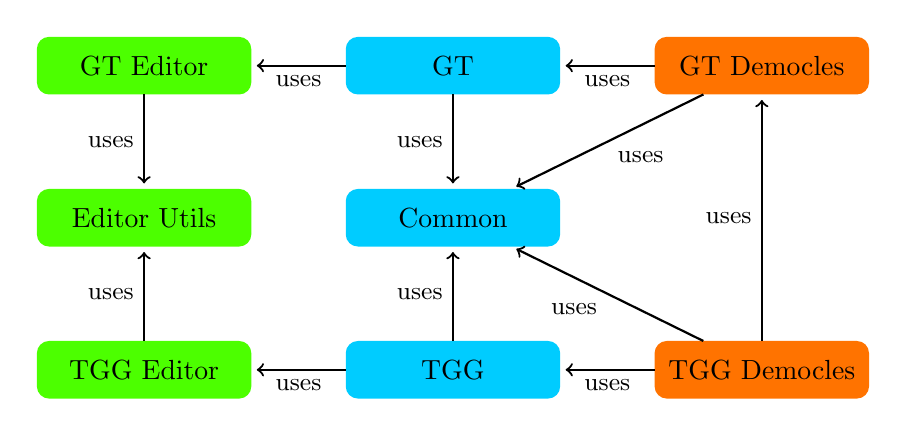
\begin{tikzpicture} [
		auto,
		node/.style = {
			rectangle,
			rounded corners,
			thick,
			text width = 7em,
			text centered,
			minimum height = 2em,
		},
		line/.style = {
			draw,
			thick,
			->,
			shorten >=2pt,
		},
		line-caption/.style = {
			font = \small,
		},
		ibex-ui/.style = {
			draw = green!60!lime,
			fill = green!60!lime,
		},
		ibex/.style = {
			draw = blue!20!cyan,
			fill = blue!20!cyan,
		},
		ibex-democles/.style = {
			draw = red!10!orange,
			fill = red!10!orange
		}
	]

	\matrix[
		column sep = 12mm,
		row sep = 12mm
	] {
		\node[node, ibex-ui] (uiGT) {
			GT Editor
		};
		& \node[node, ibex](GT) {
			GT
		};
		& \node[node, ibex-democles](democlesGT) {
			GT Democles
		};
		\\
		\node[node, ibex-ui] (uiCommon) {
			Editor Utils
		};
		& \node[node, ibex](common) {
			Common
		};
		\\
		\node[node, ibex-ui] (uiTGG) {
			TGG Editor
		};
		& \node[node, ibex](TGG) {
			TGG
		};
		& \node[node, ibex-democles](democlesTGG) {
			TGG Democles
		};
		\\
	};

	\begin{scope} [
		every path/.style = line,
		every node/.style = line-caption
		]
		\path (uiGT) -- node[left] {uses} (uiCommon);
		\path (uiTGG) -- node[left] {uses} (uiCommon);

		\path (GT) -- node {uses} (uiGT);
		\path (TGG) -- node {uses} (uiTGG);

		\path (GT) -- node[left] {uses} (common);
		\path (TGG) -- node[left] {uses} (common);

		\path (democlesGT) -- node {uses} (GT);
		\path (democlesGT) -- node {uses} (common);
		\path (democlesTGG) -- node {uses} (common);
		\path (democlesTGG) -- node {uses} (TGG);
		\path (democlesTGG) -- node {uses} (democlesGT);
	\end{scope}
\end{tikzpicture}

	\caption[Component Diagram for eMoflon::IBeX]{Component Diagram for eMoflon::IBeX (see Appendix~\ref{appendix-list-of-projects} for details)}
	\label{fig:emoflon-ibex-components}
\end{figure}

\noindent
The Common project defines the meta-model for IBeX pattern model, a pattern network which is independent from a concrete pattern matcher.
Currently IBeX patterns are used for GT only, but shall be shared with the TGG part later.
In addition, some utilities for dealing with EMF models are provided.

The GT and TGG projects provide Eclipse integration and runtime code which is independent from a concrete pattern matcher.
To use eMoflon::IBeX, an adapter for a concrete incremental pattern matching engine is necessary.
Currently only Democles \cite{Democles} is fully supported, although prototypes for Viatra and Drools exist.


\section{Transformation of Graph Transformation Rules into IBeX Patterns}
\label{ibex-patterns}
This section explains the transformation from the textual specification in the editor into IBeX patterns which can be understood by a pattern matching engine after another transformation into the pattern format of the engine.
In the following, patterns and rules will be given by their textual syntax and graphical visualization.
The interested reader is referred to the handbook \cite{eMoflonIBeX-GT-Handbook} for more details about the textual syntax.

Figure~\ref{fig:model-transformations} illustrates the use of model transformations in the eMoflon::IBeX implementation.
The user specifies patterns and rules in text files with the file extension \texttt{gt} using an Xtext-based editor.
Xtext automatically parses the file and transforms the textual specification into an editor model when a \texttt{gt} file is loaded.

The visualizations of the editor model, the IBeX patterns, and the Democles patterns are realized via transformations to PlantUML code, which is interpreted and displayed by the PlantUML Eclipse plugin.

\begin{figure}[h!]
	\centering
	% !TeX encoding = UTF-8
% !TeX spellcheck = en_US

\begin{tikzpicture} [
		auto,
		node distance = 2.25cm,
		node/.style = {
			rectangle,
			rounded corners,
			thick,
			text width = 6em,
			text centered,
			minimum height = 3em,
		},
		line/.style = {
			draw,
			thick,
			->,
			shorten >=2pt,
		},
		line-caption/.style = {
			font = \footnotesize
		},
		ibex-ui/.style = {
			draw = green!60!lime,
			fill = green!60!lime,
		},
		ibex/.style = {
			draw = blue!20!cyan,
			fill = blue!20!cyan,
		},
		ibex-democles/.style = {
			draw = red!10!orange,
			fill = red!10!orange
		}
	]

	\node[node, ibex-ui] (f) {
		\texttt{gt} text file
	};

	\node[node, ibex-ui, below of = f] (e) {
		Editor Model
	};
	\node[node, ibex-ui, left = 2cm of e] (ev) {
		Editor Model Visualization
	};
	\node[node, ibex-ui, right = 2cm of e] (em) {
		Xtext-based Meta-Model
	};

	\node[node, ibex, below of = e, xshift = 1.6cm] (g) {
		GT API Model
	};
	\node[node, ibex, right = 2cm of g] (gm) {
		GT API Meta-Model
	};
	\node[node, ibex, below of = g] (gc) {
		Java API
	};

	\node[node, ibex, below of = e, xshift = -1.6cm] (i) {
		IBeX Patterns
	};
	\node[node, ibex, left = 2cm of i] (im) {
		IBeX Pattern Meta-Model
	};
	\node[node, ibex, below of = i] (iv) {
		IBeX Pattern Visualization
	};

	\node[node, ibex-democles, below of = im] (d) {
		Democles Patterns
	};
	\node[node, ibex-democles, below of = d] (dm) {
		Democles Meta-Model
	};
	\node[node, ibex-democles, below of = iv] (dv) {
		Democles Visualization
	};

	\begin{scope} [
			every path/.style = line, ibex-ui,
			every node/.style = line-caption
		]
		\path (f) -- node[right] {Xtext transformation} (e);
		\path (e) -- node[below] {visualized in} (ev);
		\path (e) -- node[below] {conforms to} (em);
	\end{scope}

	\begin{scope} [
			every path/.style = line, ibex,
			every node/.style = line-caption
		]
		\path (e) -- node[left, xshift = -0.2cm] {transformation} (i.north);
		\path (e) -- node[right, xshift = 0.2cm] {transformation} (g.north);

		\path (i) -- node[below] {conforms to} (im);
		\path (i) -- node[right] {visualized in} (iv);

		\path (g) -- node[below] {conforms to} (gm);
		\path (g) -- node[right] {code generation} (gc);
	\end{scope}

	\begin{scope} [
			every path/.style = line, ibex-democles,
			every node/.style = line-caption
		]
		\path (i) -- node[left, yshift = 0.2cm] {transformation} (d.east);
		\path (d) -- node[right] {conforms to} (dm);
		\path (d) -- node[right, xshift = 0.2cm] {visualized in} (dv);
	\end{scope}
\end{tikzpicture}

	\caption{Model transformations for eMoflon::IBeX-GT}
	\label{fig:model-transformations}
\end{figure}

\noindent
Whenever a project with \texttt{gt} files is built, the editor models of all \texttt{gt} files in a package are transformed into the GT API model and the IBeX pattern model.
In addition, code for a typed Java API is generated as described in Section~\ref{api-code-generation}.

For each pattern and each rule a context pattern containing all context elements, deleted elements, and attribute conditions is generated.
In addition, for each rule a create and a delete pattern is generated to define which elements must be created or deleted when the rule is applied.
The create pattern contains all created nodes and references, together with any attribute assignments, while a delete pattern contains just deleted nodes and references.
Figure~\ref{fig:editor-model-to-IBeXPatterns} summarizes which parts of the editor model are included in which kind of the generated IBeX patterns.

\begin{figure}[h!]
	\centering
	\input{../common/tikz/editor-model-to-IBeXPatterns.tex}
	\caption{Editor model to IBeX patterns}
	\label{fig:editor-model-to-IBeXPatterns}
\end{figure}

\noindent
The transformation from IBeX context patterns to the pattern representation used by a concrete incremental pattern matching engine (\eg Democles) happens at runtime.
If one wants to use eMoflon::IBeX with another pattern matcher, just the orange part in Figure~\ref{fig:model-transformations} (the Democles adapter) needs to be implemented for the other engine, as just this part depends on the meta-model for Democles patterns.

\subsection{Nodes and References}
A pattern/rule consists of nodes and references between them.
Each node and reference must have a type from an Ecore meta-model.
The type of a node can be abstract -- except if the node is created and the rule is not abstract (cp. Section~\ref{pattern-refinement}).
This ensures that all created nodes in applicable rules have a concrete type such that the node can be actually created, which would not be possible for an abstract type.

For each node and reference an operator defines whether it is context (shown with black background in the visualization), created (green) or deleted (red).
Note that some combinations of node and reference operator do not make sense and are forbidden, \eg there must not be a context reference in a created node as there cannot be a reference in a node which does not exist yet.

The pattern \texttt{findCharacterOnExit} (Figure~\ref{fig:pattern-findCharacterOnExit}) will match any characters standing on an exit platform.
The rule \texttt{createCharacter} (Figure~\ref{fig:rule-createCharacter}) which creates a new character and references from the character to an existing game and to an existing platform.
The rule \texttt{moveCharacterToNeighboringPlatform} (Figure~\ref{fig:rule-moveCharacterToNeighboringPlatform}) deletes the \texttt{standsOn} reference between a character to its current platform and creates a new \texttt{standsOn} reference to another platform which must be a neighbor of the previous one.

\begin{figure}[h!]
	\centering
	\subfloat[Textual Syntax]{
		\includegraphics{../common/figures/pattern-findCharacterOnExit-textual}
	}
	\quad
	\subfloat[Visualization]{
		\includegraphics[scale=0.7]{../common/figures/pattern-findCharacterOnExit}
	}
	\caption{Pattern \texttt{findCharacterOnExit}}
	\label{fig:pattern-findCharacterOnExit}
\end{figure}

\begin{figure}[h!]
	\centering
	\subfloat[Textual Syntax]{
		\includegraphics{../common/figures/rule-createCharacter-textual}
	}
	\quad
	\subfloat[Visualization]{
		\includegraphics[scale=0.7]{../common/figures/rule-createCharacter}
	}
	\caption{Rule \texttt{createCharacter}}
	\label{fig:rule-createCharacter}
\end{figure}

\begin{figure}[h!]
	\centering
	\subfloat[Textual Syntax]{
		\includegraphics{../common/figures/rule-moveCharacterToNeighboringPlatform-textual}
	} \\
	\subfloat[Visualization]{
		\includegraphics[scale=0.7]{../common/figures/rule-moveCharacterToNeighboringPlatform}
	}
	\caption{Rule \texttt{moveCharacterToNeighboringPlatform}}
	\label{fig:rule-moveCharacterToNeighboringPlatform}
\end{figure}

\noindent
In eMoflon::IBeX matches must be injective, \ie nodes with different names must be matched to different objects in a match. 
For example, the two platforms in the rule \texttt{moveCharacterToNeighboringPlatform} must be different platforms.
So a platform which has a \texttt{neighbors} edge to itself would not be a valid match.
The decision for injectivity per default has been made as this is what the user intuitively expects when looking at the visualization.
If one does not want to have injectivity for a pattern, one has to specify different variants of the pattern.

A match for a pattern contains all nodes of that pattern -- except so-called local nodes.
Per convention in eMoflon::IBeX-GT, a node is local if and only if its name starts with an underscore.
If one was not interested in the platforms of Figure~\ref{fig:rule-moveCharacterToNeighboringPlatform}, one could name them \texttt{\_platform1} and \texttt{\_platform2} to omit them from in the matches for the pattern.
So local nodes can be used to get smaller matches, as less elements are contained in the match.
As the binding of local nodes is not relevant for the match, specifying nodes as local can reduce the number of matches because different bindings for the local nodes do not result in different matches.

\subsection{Attribute Assignments and Conditions}
Attribute assignments define new attribute values to be set when the rule is applied, 
while attribute conditions are a match filter based on a comparison of attribute values according to the defined relation (\texttt{==}, \texttt{!=}, \texttt{<=}, \texttt{<}, \texttt{>}, or \texttt{>=}).
eMoflon::IBeX-GT supports constants, the attributes of other nodes, and parameters as attribute values as long as the type of the value fits to the one of the attribute.
For example, a String attribute can only have a String value.

\begin{figure}[h!]
	\centering
	\subfloat[Textual Syntax]{
		\includegraphics{../common/figures/pattern-findCharacterOfColor-textual}
	}
	\quad
	\subfloat[Visualization]{
		\includegraphics[scale=0.7]{../common/figures/pattern-findCharacterOfColor}
	}
	\caption{Pattern \texttt{findCharacterOfColor(color: COLOR)}}
	\label{fig:pattern-findCharacterOfColor}
\end{figure}

\begin{figure}[h!]
	\centering
	\subfloat[Textual Syntax]{
		\includegraphics{../common/figures/rule-createBlueCharacter-textual}
	}
	\quad
	\subfloat[Visualization]{
		\includegraphics[scale=0.7]{../common/figures/rule-createBlueCharacter}
	}
	\caption{Rule \texttt{createBlueCharacter}}
	\label{fig:rule-createBlueCharacter}
\end{figure}

\noindent
The pattern \texttt{findColoredCharacter} (Figure~\ref{fig:pattern-findCharacterOfColor}) searches for a character which stands on a platform and has a certain color.
The attribute condition defines that only characters whose color attribute equals the value of the parameter \texttt{color} of the type \texttt{COLOR} (an enum defined in the meta-model) can be matched.
The rule \texttt{createBlueCharacter} (Figure~\ref{fig:rule-createBlueCharacter}) creates a new character whose color attribute is set to \texttt{BLUE}, given by an enum literal.
Attributes which are not specified for created nodes are set to the default value defined in the Ecore meta-model.

Parameters for primitive data types and enums must be declared in the signature of a pattern or a rule.
At run time they are replaced with a concrete value of the correct type.\footnote{Section~\ref{api-parameters} explains how parameters can be passed via the API.}
As parameter values are only bound at run time, parameterized attribute conditions cannot be transformed to Democles, but are handled by the graph transformation interpreter.

Note that there are some logical restrictions when using attribute assignments and conditions:
Attribute assignments must not be placed in deleted nodes (if the node was deleted, its attributes cannot be changed anymore) and conditions cannot occur within created nodes (the node does not exist yet and does not have any attribute values).

\subsection{Applications Conditions}
\label{application-conditions}
Application conditions are additional constraints on graph structures to check when finding matches for a certain pattern:
The application conditions must be fulfilled for the match according to Definitions~\ref{def:satisfaction-of-graph-conditions} and~\ref{def:satisfaction-of-complex-graph-conditions}, otherwise the match is not valid.
eMoflon::IBeX-GT allows to specify positive and negative application conditions and combine them via logical expressions \texttt{\&\&} (logical conjunction) and \texttt{||} (logical disjunction).

By convention, nodes of the same name in a pattern and the patterns used in its application conditions must be matched to the same node.
The arrows in the visualization illustrate which nodes of the different patterns must be equal.
Only the nodes of the main pattern are included in matches, any bindings of the nodes in the patterns of conditions will not be available in matches.

\subsubsection{Negative Application Conditions}
Via \texttt{forbid} a negative application condition (NAC) can be defined.
A NAC invalidates matches with a certain pattern structure.
For example, the pattern \texttt{findEmptyExit} (Figure~\ref{fig:pattern-findEmptyExit}) contains a NAC to ensure that no character stands on the exit platform of the main pattern.
Otherwise any exit platform could be mapped for the \texttt{exit} node regardless of whether characters stand on it or not.

\begin{figure}[h!]
	\centering
	\subfloat[Textual Syntax]{
		\includegraphics{../common/figures/pattern-findEmptyExit-textual}
	}
	\caption{Pattern \texttt{findEmptyExit}}
	\label{fig:pattern-findEmptyExit}
\end{figure}

\begin{figure}[h!]
	\centering
	\ContinuedFloat
	\subfloat[Visualization]{
		\includegraphics[scale=0.7]{../common/figures/pattern-findEmptyExit}
	}
	\caption[]{Pattern \texttt{findEmptyExit} (cont.)}
\end{figure}

\begin{figure}[h!]
	\centering
	\subfloat[Textual Syntax]{
		\includegraphics{../common/figures/pattern-findStandalonePlatform-textual}
	}
	\caption{Pattern \texttt{findStandalonePlatform}}
	\label{fig:pattern-findStandalonePlatform}
\end{figure}

\begin{figure}[h!]
	\ContinuedFloat
	\centering
	\subfloat[Visualization]{
		\includegraphics[scale=0.7]{../common/figures/pattern-findStandalonePlatform}
	}
	\caption[]{Pattern \texttt{findStandalonePlatform} (cont.)}
\end{figure}

\noindent
Multiple application conditions can be combined via \texttt{\&\&} as illustrated in the pattern \texttt{findStandalonePlatform} (Figure~\ref{fig:pattern-findStandalonePlatform}).
The two NACs restrict the matches for the simple platforms such that all platforms which are connected to another platform via a bridge or a wall are excluded as well as any platforms with a neighboring platform.
Platforms matched by the pattern \texttt{findStandalonePlatform} cannot be left by a character standing on it.
When a She Remembered Caterpillars world is created, such a standalone platform with a character standing on it should be avoided, otherwise the game cannot be finished.

\subsubsection{Positive Application Conditions}
The pattern \texttt{findPlatformWithExactlyOneNeighbor} (Figure~\ref{fig:pattern-findPlatformWithExactlyOneNeighbor}) uses a positive application condition (PAC) via \texttt{enforce} in combination with a NAC.
The PAC ensures that the platform must have at least one neighboring platform and the NAC excludes any platforms which have at least two neighbors.
Finally, only the platforms with exactly one neighbor remain as matches.

In this example, the PAC could be simply integrated into the main pattern without changing its meaning.
However, in general PACs are necessary to express certain constraints:
For example, multiple PACs combined via disjunction cannot be expressed with the integration into the main pattern (cp. example in Section \ref{disjunctions}).
In addition, the nodes used in application conditions are not contained in the matches.

\begin{figure}[h!]
	\centering
	\subfloat[Textual Syntax]{
		\includegraphics{../common/figures/pattern-findPlatformWithExactlyOneNeighbor-textual}
	} \\
	\subfloat[Visualization]{
		\includegraphics[scale=0.7]{../common/figures/pattern-findPlatformWithExactlyOneNeighbor}
	}
	\caption{Pattern \texttt{findPlatformWithExactlyOneNeighbor}}
	\label{fig:pattern-findPlatformWithExactlyOneNeighbor}
\end{figure}

\subsubsection{Disjunctions}
\label{disjunctions}
Application conditions can be used to express alternatives as well:
For example,
the pattern \texttt{findPlatformWithTwoWays} (Figure~\ref{fig:pattern-findPlatformWithTwoWays}) searches for platforms which have at least two ways to enter or leave the platform (either via neighboring platforms or via bridges/walls).
To express this, three application conditions need to be combined via \texttt{||} to deal with the possibilities that the platform 
(1) has two neighboring platforms,
(2) has two connections to bridges or walls,
or (3) one neighboring platform and one connection to a bridge or a wall.

\begin{figure}[h!]
	\centering
	\subfloat[Textual Syntax]{
		\includegraphics{../common/figures/pattern-findPlatformWithTwoWays-textual}
	}
	\caption{Pattern \texttt{findPlatformWithTwoWays}}
	\label{fig:pattern-findPlatformWithTwoWays}
\end{figure}

\begin{figure}
	\ContinuedFloat
	\centering
	\subfloat[Visualization]{
		\includegraphics[width=\linewidth, trim=8mm 0 0 0]{../common/figures/pattern-findPlatformWithTwoWays-ltr}
	}
	\caption[]{Pattern \texttt{findPlatformWithTwoWays} (cont.)}
\end{figure}

\noindent
In the IBeX pattern model, patterns with multiple disjunctions are represented as a set of alternative patterns.
A match for the pattern is defined as a match for any of the alternative patterns.
For each alternative pattern a separate pattern is generated which is given to the pattern matching engine because Democles cannot deal with alternatives directly (although this feature is planned for the future).
As usual, Democles reports the matches for all patterns to the graph transformation interpreter, which has to collect and combine the matches of all alternative patterns, excluding duplicate matches.
The removal of duplicates is necessary as Democles may report the same match for multiple alternative patterns.

The three alternatives for the pattern \texttt{findPlatformWithTwoWays} are disjoint.
So no matches will be removed when combining the matches of the three alternatives because no duplicates can be found.
Without the NACs in the third alternative, a match for a platform with two neighbors and a bridge connection (as the platform \texttt{p1} shown in Figure~\ref{fig:example-model-duplicate-matches}) would be reported by the first and the third alternative.
The duplicate check would remove one of the matches, so the interpreter would still return the same set of matches.
Without the removal of matches, a match reported by two alternatives would be returned twice.

\begin{figure}[h!]
	\centering
	\begin{tikzpicture}
		\node[tnode] (p1) {p1: SimplePlatform};
		\node[tnode, below = of p1] (p2) {p2: SimplePlatform};
		\node[tnode, left = of p2] (b) {b: Bridge};
		\node[tnode, right = of p2] (p3) {p3: SimplePlatform};
		
		\draw[tedge] (p1.west) -- (b);
		\draw[tedge] (p2) -- (b);
		\draw[tedge] (p1) -- (p2);
		\draw[tedge] (p1) -- (p3);
	\end{tikzpicture}
	\caption{Example Model with Matches Reported for Two Alternatives}
	\label{fig:example-model-duplicate-matches}
\end{figure}

\noindent
Note that logical expressions combining application conditions must be given in disjunctive normal form (DNF), \ie the clauses combined via \texttt{||} must only contain PACs and NACs combined via \texttt{\&\&}.
This is necessary to easily create the alternative patterns which can be given to the pattern matcher, as for each clause an alternative pattern is generated, containing the main pattern with the PACs and NACs from the clause.

\subsection{Pattern Refinement}
\label{pattern-refinement}
Pattern refinement is a modularity concept on the level of patterns which allows to share common subparts of the pattern with one or multiple super patterns.
Similar to inheritance in object-oriented programming, this avoids declaring the same graph structures in multiple patterns.
So pattern refinement helps to reduce copy and paste and leads to a specification which can be maintained more easily.

Patterns with super patterns are flattened, \ie transformed into an equivalent version without pattern refinement.
After that the flattened pattern is transformed into IBeX patterns as shown in Figure~\ref{fig:editor-model-to-IBeXPatterns}.
The semantics of pattern refinement (how a pattern with super patterns can be flattened) is given by Definition~\ref{def:refined-pattern}.\footnote{The definition of rule refinement for Triple Graph Grammars by Stolte \cite{ExploitingTheModularityOfTGGs} is generalized for graph transformations.}
Note that application conditions are not inherited to avoid additional complexity in situations in which the application conditions of super patterns come into conflict with each other.
Due to this decision the user cannot lose track of the application conditions of a concrete pattern.

Patterns can be abstract: Abstract means that the pattern cannot be applied directly, but only exists to be used as a super pattern.

\newpage % Without this line LaTeX puts a pagebreak after the first line of the definition.
\begin{definition}[Refined Pattern]
	\label{def:refined-pattern}%
	A pattern with one or more super patterns is called a \textit{refined pattern}.
	The semantics of such a pattern is defined by the following constraints:
	\begin{enumerate}
		\item A pattern contains all nodes from its super patterns.
		\item Equivalent nodes (identified by their name) are merged into one node.
		\item Equivalent references (identified by their type, source and target node) are merged into one edge.
		\item Equivalent attribute assignments (identified by their node, attribute type and value) are merged into one attribute assignment.
			There must not be different attribute assignments for the same attribute inherited from different patterns.
		\item Equivalent attribute conditions (identified by their node, attribute type, relation and value) are merged into one attribute condition.
		\item Equivalent parameters (identified by their name) are merged into one parameter.
			There must not be different type definitions for parameters of the same name.
		\item When overriding a node/reference, created/deleted elements can be overwritten by context elements.
			Context elements must not be overwritten by created or deleted elements.
			Created elements must not be overwritten by deleted elements, deleted elements must not be overwritten by created elements.
		\item The type of a node is the lowest of the types of all declarations of a node within a pattern and its super patterns.
			The type of a node can only be the same type or a lower type as declared for a node of the same name in a super pattern.
	\end{enumerate}
\end{definition}

\noindent
Table~\ref{table:node-type-changes} shows some combinations of allowed and forbidden node type declarations in refined patterns and their super patterns according to the last constraint.
Specifications without a lowest type and type not conforming to the type in the super pattern lead to an error message in the editor.

\begin{longtable}[h!]{lll}
	\toprule
	Node types in super patterns
		& Node type in pattern
		& Final type \\
	\midrule
	Platform
		& \text{(none)}
		& Platform \\
	Platform, SimplePlatform
		& (none)
		& SimplePlatform \\
	ExitPlatform, SimplePlatform
		& (none)
		& ERROR (no lowest type) \\
	ExitPlatform
		& Platform
		& ERROR (no subtype) \\
	Platform
		& SimplePlatform
		& SimplePlatform \\
	ExitPlatform
		& SimplePlatform
		& ERROR (no subtype) \\
	\bottomrule
	\caption{Allowed and Forbidden Node Type Changes in Refined Patterns}
	\label{table:node-type-changes}
\end{longtable}

\begin{figure}[h!]
	\centering
	\subfloat[Textual Syntax]{
		\includegraphics{../common/figures/rules-moveCharacter-textual}
		\label{fig:rules-moveCharacter-textual}
	}
	\caption{Rules with Refinements}
	\label{fig:examples-with-refinement}
\end{figure}

\begin{figure}[h!]
	\ContinuedFloat
	\centering
	\subfloat[Refinement Hierarchy]{
		\includegraphics{../common/figures/pattern-refinement-hierarchy-moveCharacter}
		\label{fig:pattern-refinement-hierarchy-moveCharacter}
	} \\
	\subfloat[Abstract Rule \texttt{moveCharacter}]{
		\includegraphics[scale=0.7]{../common/figures/rule-moveCharacter}
		\label{fig:rule-moveCharacter}
	}
	\subfloat[Rule \texttt{moveCharacterToNeighboringPlatform}]{
		\includegraphics[scale=0.7]{../common/figures/rule-moveCharacterToNeighboringPlatform}
		\label{fig:rule-moveCharacterToNeighboringPlatform2}
	}
	\caption[]{Rules with Refinements (cont.)}
\end{figure}

\noindent
Figure~\ref{fig:examples-with-refinement} shows some rules having a lot of elements in common.
Using the pattern refinement hierarchy shown in Figure~\ref{fig:pattern-refinement-hierarchy-moveCharacter}, duplications in the textual specification can be avoided or at least significantly reduced as only nodes with additional references or another type need to be redeclared in the refined pattern.
Nodes which are already defined in a super pattern are highlighted in bold.
The visualization shows the refined rules after the flattening according to Definition~\ref{def:refined-pattern}.

The rule \texttt{moveCharacterToNeighboringPlatform} just specifies the \texttt{neighbors} edge between the two platforms, all objects and the other edges are inherited from the super rule \texttt{moveCharacter}.
The abstract rule \texttt{moveCharacterAcrossPlatformConnector} overrides the type of the platform nodes to a subtype, \texttt{SimplePlatform}.
The rules \texttt{moveCharacterAcrossBridge} and \texttt{moveCharacterOverWall} define that the two platforms must be connected via a bridge or a wall, respectively.

\begin{figure}[h!]
	\ContinuedFloat
	\centering
	\subfloat[Abstract Rule \texttt{moveCharacterAcrossPlatformConnector}]{
		\includegraphics[scale=0.7]{../common/figures/rule-moveCharacterAcrossPlatformConnector}
		\label{fig:rule-moveCharacterAcrossPlatformConnector}
	} \\
	\subfloat[Rule \texttt{moveCharacterAcrossBridge}]{
		\includegraphics[scale=0.7]{../common/figures/rule-moveCharacterAcrossBridge}
		\label{fig:rule-moveCharacterAcrossBridge}
	} \\
	\subfloat[Rule \texttt{moveCharacterOverWall}]{
		\includegraphics[scale=0.7]{../common/figures/rule-moveCharacterOverWall}
		\label{fig:rule-moveCharacterOverWall}
	}
	\caption[]{Rules with Refinements (cont.)}
\end{figure}

The algorithm for the flattening of an editor pattern collects all nodes of the pattern and its super patterns and combines them into one large pattern (so-called co-product).
After that parts which are equivalent according to Definition~\ref{def:refined-pattern} are merged as described in the following:

\begin{enumerate}
	\item When merging two nodes, the operator is given by Table~\ref{table:merging-operators} (see constraint 7 in the definition) and the type of the node is the lower type of the two merged nodes.
		In the case that two nodes of the same name have different types and none of the types is a subtype of the other, the specification is invalid.
	\item When merging two equivalent references, attribute assignments, or attribute conditions only one of them remains and the other one is removed.
		\begin{enumerate}
			\item The operator of merged references is given by Table~\ref{table:merging-operators}.
			\item If there are multiple attribute assignments for the same attribute within a node, their values must be equal.
				Otherwise the specification is invalid, as one cannot decide which attribute value shall be assigned.
		\end{enumerate}
	\item When merging parameters, the parameters of the super patterns are appended to the parameter list of the refined pattern.
		If parameters of the same name have different types, the specification is invalid.
\end{enumerate}

\begin{longtable}[h!]{c|ccc}
	\toprule
				& \create	& \delete 	& context \\
	\midrule
	\create		& \create	& ERROR		& context \\
	\delete		& ERROR		& \delete	& context \\
	context		& context	& context	& context \\
	\bottomrule
	\caption{Operators of Merged Nodes and References in Refined Patterns}
	\label{table:merging-operators}
\end{longtable}

\noindent
For the flattening algorithm it is irrelevant whether a node is specified in the refined pattern or one of its super patterns.
Only for parameters the order is relevant (because the parameters of the pattern specification become parameters for the constructor of the pattern).
By repeating all parameters in the refined pattern, the user can influence the order of all parameters.

The user gets feedback on invalid specifications by error markers shown in the editor.
When a project with invalid specifications is built, the problems are written on the console.


\section{Pattern Networks}
\label{pattern-networks}
The previous sections introduced the features of the pattern language in the textual editor: nodes and references, attributes, application conditions, and pattern refinement.
This section gives a summary how they are represented in the editor model, the IBeX pattern model, and in Democles.
In addition, details on the transformations are provided.

The parser of the Xtext framework parses \texttt{gt} files into an editor model file containing \texttt{EditorPattern}s and \texttt{EditorCondition}s.
Figure~\ref{fig:editor-patterns-meta-model} shows a simplified class diagram of the editor model.
\texttt{EditorPattern}s have a type, either \texttt{PATTERN} or \texttt{RULE}.
By using the same object for patterns and rules, both can easily be used together in a refinement hierarchy.
They consist of a set of \texttt{EditorNode}s, which can have \texttt{EditorAttribute}s and \texttt{EditorReference}s.
An \texttt{EditorAttribute} has a relation (assignment or a comparison such as equals) and an attribute value.
An \texttt{EditorReference} has a target node.

Both \texttt{EditorNode}s and \texttt{EditorReference}s have an operator, either \texttt{CONTEXT} (default value), \texttt{CREATE} (keyword \create~in the editor), or \texttt{DELETE} (\delete).

\texttt{EditorPattern}s have a set of \texttt{EditorCondition}s (disjunction).
\texttt{EditorCondition}s represent a conjunction of conditions (a clause in the DNF), which can be a reference to another \texttt{EditorCondition} or a positive or negative \texttt{EditorApplicationCondition} (\texttt{enforce} or \texttt{forbid}).
\texttt{EditorConditionReference} reference another condition.

\begin{figure}[H]
	\centering
	% !TeX encoding = UTF-8
% !TeX spellcheck = en_US

\begin{tikzpicture}
	\umlsimpleclass[class]
		{EditorPattern}

	% classes for conditions
	\umlsimpleclass[class,
		below = 1.5cm of EditorPattern,
		xshift = -2cm]
		{EditorCondition}
	\umlsimpleclass[class,
		below = 1.5cm of EditorCondition]
		{EditorSimpleCondition}
	\umlsimpleclass[class,
		below = 2.25cm of EditorSimpleCondition,
		xshift = 2cm]
		{EditorConditionReference}
	\umlsimpleclass[class,
		below = 1cm of EditorSimpleCondition,
		xshift = -2cm]
		{EditorApplicationCondition}

	% classes node, attribute and reference
	\umlsimpleclass[class,
		below = 1.5cm of EditorPattern,
		xshift = 4.25cm]
		{EditorNode}
	\umlsimpleclass[class,
		below = 1.5cm of EditorNode,
		xshift = -1.8cm]
		{EditorAttribute}
	\umlsimpleclass[class,
		below = 1.5cm of EditorNode,
		xshift = 1.8cm]
		{EditorReference}

	% EditorPattern
	\umluniassoc[arg2 = {superPatterns},
		mult2 = 0..*,
		pos = 0.5,
		angle1 = 90,
		angle2 = 0,
		loopsize = 2cm]
		{EditorPattern}
		{EditorPattern}
	\umluniassoc[geometry=|-|,
		arg2 = {conditions (OR)},
		mult2 = 0..*,
		pos2 = 2.5,
		anchor1 = -130,
		anchor2 = 90]
		{EditorPattern}
		{EditorCondition}
	\umlunicompo[geometry = |-|,
		arg2 = {nodes},
		mult2 = 0..*,
		pos = 2.5,
		anchor1 = -50,
		anchor2 = 90]
		{EditorPattern}
		{EditorNode}

	% EditorNode
	\umlunicompo[geometry = |-|,
		arg2 = {attributes},
		mult2 = 0..*,
		pos = 2.5,
		anchor1 = -130]
		{EditorNode}
		{EditorAttribute}
	\umlunicompo[geometry = |-|,
		arg2 = {references},
		mult2 = 0..*,
		pos = 2.5,
		anchor1 = -50,
		anchor2 = 90]
		{EditorNode}
		{EditorReference}

	% EditorReference
	\umluniassoc[geometry = -|-,
		arg2 = {target},
		mult2 = 1,
		pos = 2.5,
		anchor1 = 0,
		anchor2 = 0,
		arm1 = 0.5cm]
		{EditorReference}
		{EditorNode}

	% EditorCondition
	\umlunicompo[arg2 = {conditions (AND)},
		mult2 = 1..*,
		pos2 = 0.75]
		{EditorCondition}
		{EditorSimpleCondition}

	% EditorConditionReference
	\umlinherit[geometry = |-|,
		anchor1 = 125,
		anchor2 = -20]
		{EditorConditionReference}
		{EditorSimpleCondition}
	\umluniassoc[geometry = |-|,
		arm1 = 1.5cm,
		arg2 = {condition},
		mult2 = 1,
		pos2 = 1.45,
		anchor1 = 12,
		anchor2 = -12]
		{EditorConditionReference}
		{EditorSimpleCondition}

	% EditorApplicationCondition
	\umlinherit[geometry = |-|,
		anchor2 = -135]
		{EditorApplicationCondition}
		{EditorSimpleCondition}
	\umluniassoc[geometry = |-,
		arg2 = {pattern},
		mult2 = 1,
		pos = 1.5,
		anchor1 = 170,
		anchor2 = 180]
		{EditorApplicationCondition}
		{EditorPattern}
\end{tikzpicture}

	\caption{Simplified Meta-Model of the Editor Model}
	\label{fig:editor-patterns-meta-model}
\end{figure}

\subsection{IBeX Pattern Networks}
\label{ibex-pattern-networks}
During the build of a graph transformation project in Eclipse with eMoflon::IBeX, the editor specification is transformed into the IBeX pattern model, which is saved in an \texttt{ibex-patterns.xmi}.
Just this file is used by the graph transformation interpreter and must be read at runtime.

A simplified class diagram for the IBeX pattern model (just context patterns) is shown in Figure~\ref{fig:ibex-patterns-meta-model}.
An \texttt{IBeXContextPattern} consists of signature nodes, local nodes and edges, injectivity constraints, attribute constraints, and pattern invocations.

Table~\ref{table:ibex-pattern-networks} summarizes how patterns and rules of the editor model are transformed into the IBeX pattern model.
\texttt{EditorPattern}s with no or just one clause in the DNF are transformed into an \texttt{IBeXContextPattern}.
If there are more than two disjunctions, the \texttt{EditorPattern} is transformed into an \texttt{IBeXContextAlternative}s, containing one \texttt{IBeXContextPattern} per clause in the DNF.

Each \texttt{EditorNode} is transformed to an \texttt{IBeXNode}.
If the name of the name starts with an underscore, the node is local (\ie not part of a match), otherwise the node is a signature node.
For each pair of two nodes for which the type declaration does not ensure that the nodes are mapped to different objects, an injectivity constraint is added.
Such a constraint defines a pair of nodes, which must not be equal.

Pattern refinement is not included in the table as the refinement is ``flattened'' and the flattened pattern is transformed afterwards.

\begin{figure}[H]
	\centering
	% !TeX encoding = UTF-8
% !TeX spellcheck = en_US

\begin{tikzpicture}
	\umlsimpleclass[class]
		{IBeXContext}
	\umlsimpleclass[class,
		right = 1.5cm of IBeXContext]
		{IBeXContextAlternatives}
	\umlsimpleclass[class,
		below = 1cm of IBeXContext]
		{IBeXContextPattern}
	\umlsimpleclass[class,
		below = 1.5cm of IBeXContextPattern,
		xshift = -4cm]
		{IBeXPatternInvocation}
	\umlsimpleclass[class,
		below = 1.5cm of IBeXContextPattern,
		xshift = 5cm]
		{IBeXAttributeConstraint}
	\umlsimpleclass[class,
		below = 0.75cm of IBeXAttributeConstraint,
		xshift = 1cm]
		{IBeXNodePair}
	\umlsimpleclass[class,
		below = 1cm of IBeXNodePair]
		{IBeXNode}
	\umlsimpleclass[class,
		below = 2.5cm of IBeXNode]
		{IBeXEdge}

	% IBeXContextAlternatives
	\umlinherit[]
		{IBeXContextAlternatives}
		{IBeXContext}
	\umlunicompo[geometry = |-,
		arg2 = {alternatives},
		mult2 = 2..*,
		pos = 1.5,
		anchor2 = 0]
		{IBeXContextAlternatives}
		{IBeXContextPattern}

	% IBeXContextPattern
	\umlinherit[]
		{IBeXContextPattern}
		{IBeXContext}
	\umlunicompo[geometry = |-|,
		arg2 = {attributeConstraints},
		mult2 = 0..*,
		pos = 2.5,
		anchor1 = -15.2]
		{IBeXContextPattern}
		{IBeXAttributeConstraint}
	\umlunicompo[geometry = |-,
		arg2 = {injectivityConstraints},
		mult2 = 0..*,
		pos = 1.5,
		anchor1 = -25]
		{IBeXContextPattern}
		{IBeXNodePair}
	\umlunicompo[geometry = |-,
		arg2 = {signatureNodes},
		mult2 = 1..*,
		pos = 1.6,
		anchor1 = -55,
		anchor2 = 165]
		{IBeXContextPattern}
		{IBeXNode}
	\umlunicompo[geometry = |-,
		arg2 = {localNodes},
		mult2 = 0..*,
		pos = 1.4,
		anchor1 = -125,
		anchor2 = 195]
		{IBeXContextPattern}
		{IBeXNode}
	\umlunicompo[geometry = |-,
		arg2 = {localEdges},
		mult2 = 0..*,
		pos = 1.4,
		anchor1 = -155]
		{IBeXContextPattern}
		{IBeXEdge}
	\umlunicompo[geometry = |-|,
		arg2 = {invocations},
		mult2 = 0..*,
		pos = 2.5,
		anchor1 = -164.8]
		{IBeXContextPattern}
		{IBeXPatternInvocation}

	% IBeXNodePair
	\umluniassoc[arg2 = {values},
		mult2 = 2,
		pos2 = 0.5]
		{IBeXNodePair}
		{IBeXNode}

	% IBeXEdge -- IBeXNode
	\umlassoc[arg1 = {outgoingEdges},
		mult1 = 0..*,
		pos1 = 0.25,
		align1 = right,
		arg2 = {sourceNode},
		mult2 = 1,
		pos2 = 0.75,
		align2 = right,
		anchor1 = 120,
		anchor2 = -120]
		{IBeXEdge}
		{IBeXNode}
	\umlassoc[arg1 = {incomingEdges},
		mult1 = 0..*,
		pos1 = 0.25,
		align1 = left,
		arg2 = {targetNode},
		mult2 = 1,
		pos2 = 0.75,
		align2 = left,
		anchor1 = 60,
		anchor2 = -60]
		{IBeXEdge}
		{IBeXNode}

	% IBeXPatternInvocation
		\umluniassoc[geometry = -|-,
			arg2 = {invokedPattern},
			mult2 = 1,
			pos = 2.5,
			anchor1 = 180,
			arm1 = 0.5cm]
		{IBeXPatternInvocation}
		{IBeXContextPattern}
\end{tikzpicture}

	\caption{Simplified Meta-Model of the IBeX Pattern Model}
	\label{fig:ibex-patterns-meta-model}
\end{figure}

\begin{longtable}[h!]{p{55mm}p{85mm}}
	\toprule
	Editor model
		& IBeX model \\
	\midrule
	\texttt{EditorNode} (if the operator is \texttt{CONTEXT} or \texttt{DELETE})
		& \texttt{IBeXNode} (as local node if the name starts with \texttt{\_}, otherwise as a signature node)
			and injectivity constraints \\
	\midrule
	\texttt{EditorReference} (if the operator is \texttt{CONTEXT} or \texttt{DELETE})
		& Positive \texttt{IBeXPatternInvocation} of an edge pattern with two signature nodes and one \texttt{IBeXEdge} \\
	\midrule
	\texttt{EditorAttribute} (if the relation is not an assignment)
		& \texttt{IBeXAttributeConstraint} (value given by a constant, a node and an attribute type or a parameter name) \\
	\midrule
	\texttt{EditorApplicationCondition}
		& \texttt{IBeXPatternInvocation} (positive invocation for PACs, negative invocation for NACs) \\
	\bottomrule
	\caption{Transformation from the Editor Model into IBeX Patterns}
	\label{table:ibex-pattern-networks}
\end{longtable}

\noindent
References and application conditions are transformed into so-called pattern invocations.
A pattern invocation is the equivalent to a method call in general programming languages.
It defines that the graph structure of invoked pattern must be matched with the mapping of nodes from the original pattern to the signature nodes of the invoked pattern.
The patterns connected via pattern invocations form a pattern network.

The context pattern generated for the rule \texttt{moveCharacterToNeighboringPlatform} (introduced in the previous section, Figure~\ref{fig:rule-moveCharacter}) is shown Figure~\ref{fig:ibex-pattern-moveCharacterToNeighboringPlatform}.
The main pattern contains only the three nodes.
The left pattern invocation ensures that there must be a \texttt{standsOn} edge between the objects mapped to the signature nodes \texttt{character} and \texttt{platform1} in the main pattern.
\texttt{platform1} and \texttt{platform2} must be connected via a \texttt{neighbors} edge to fulfill the right pattern invocation.

Extracting the edges into edge patterns invoked by the main patterns leads to smaller patterns.
Of course, edge patterns can be invoked by multiple patterns (or even multiple times by the same pattern, using different node mappings).
For example, the edge pattern \texttt{edge-Character-standsOn-Platform} is invoked by all patterns which require a \texttt{standsOn} edge between a character and a platform.

\begin{figure}[h!]
	\centering
	\includegraphics[scale=0.7]{../common/figures/ibex-pattern-moveCharacterToNeighboringPlatform}
	\caption{IBeX Context Pattern \texttt{moveCharacterToNeighboringPlatform}}
	\label{fig:ibex-pattern-moveCharacterToNeighboringPlatform}
\end{figure}

\subsection{Democles Pattern Networks}
\label{democles-pattern-networks}
The meta-model of the pattern network used by Democles is shown in Figure~\ref{fig:democles-patterns-meta-model} (simplified).
A Democles \texttt{Pattern} consists of symbolic parameters and a \texttt{PatternBody}, which contains local variables and constraints.

All elements from the IBeX representation to their equivalent in the Democles model, as shown in Table~\ref{table:pattern-networks}.
As Democles cannot handle parameterized attribute conditions and alternatives of multiple patterns, these two scenarios are handled by the interpreter via filtering and combining (see Section~\ref{api-usage} for detailed information).

\begin{figure}[H]
	\centering
	% !TeX encoding = UTF-8
% !TeX spellcheck = en_US

\begin{tikzpicture}
	\umlsimpleclass[class]
		{Pattern}
	\umlsimpleclass[class,
		below = 1.5cm of Pattern]
		{PatternBody}
	\umlsimpleclass[class,
		below = 1.5cm of PatternBody]
		{Constraint}

	\umlsimpleclass[class,
		below = 1cm of Constraint,
		xshift = -1.5cm]
		{PatternInvocationConstraint}
	\umlsimpleclass[class,
		right = 0.5cm of PatternInvocationConstraint]
		{Reference}
	\umlsimpleclass[class,
		right = 0.5cm of Reference]
		{RelationalConstraint}
	\umlsimpleclass[class,
		below = 1cm of RelationalConstraint]
		{Unequal}
	\umlsimpleclass[class,
		left = 0.5cm of Unequal]
		{Equal}
	\umlsimpleclass[class,
		right = 0.5cm of Unequal,
		alias=x]
		{...}

	\umlsimpleclass[class,
		right = 4cm of Pattern]
		{EMFVariable}
	\umlsimpleclass[class,
		right = 4cm of Constraint]
		{ConstraintParameter}

	\umlunicompo[arg2 = {bodies},
		mult2 = 1..*,
		pos = 0.75]
		{Pattern}
		{PatternBody}
	\umlunicompo[arg2 = {symbolicParameters},
		mult2 = 1..*,
		pos = 0.5]
		{Pattern}
		{EMFVariable}
	\umlunicompo[geometry = -|,
		arg2 = {localVariables},
		mult2 = 0..*,
		pos = 0.5,
		anchor2 = -140]
		{PatternBody}
		{EMFVariable}
	\umlunicompo[arg2 = {constraints},
		mult2 = 0..*,
		pos = 0.75]
		{PatternBody}
		{Constraint}
	\umlunicompo[arg2 = {parameters},
		mult2 = 0..*,
		pos = 0.5]
		{Constraint}
		{ConstraintParameter}
	\umluniassoc[geometry = |-|,
		arg2 = {reference},
		mult2 = 0..*,
		pos = 0.75,
		anchor2 = -40]
		{ConstraintParameter}
		{EMFVariable}

	\umluniassoc[geometry = |-,
		arg2 = {invokedPattern},
		mult2 = 0..*,
		pos = 1.5,
		anchor1 = 170,
		anchor2 = 180]
		{PatternInvocationConstraint}
		{Pattern}

	\umlinherit[geometry=|-|]
		{PatternInvocationConstraint}
		{Constraint}
	\umlinherit[geometry=|-|]
		{RelationalConstraint}
		{Constraint}
	\umlinherit[geometry=|-|]
		{Reference}
		{Constraint}
	\umlinherit[geometry=|-|]
		{Equal}
		{RelationalConstraint}
	\umlinherit[geometry=|-|]
		{Unequal}
		{RelationalConstraint}
	\umlinherit[geometry=|-|]
		{x}
		{RelationalConstraint}
\end{tikzpicture}

	\caption{Simplified Meta-Model for Democles Patterns}
	\label{fig:democles-patterns-meta-model}
\end{figure}

\begin{longtable}[h!]{p{75mm}p{65mm}}
	\toprule
	IBeX model
		& Democles model \\
	\midrule
	\texttt{IBeXNode} as local node
		& \texttt{EMFVariable} as local node \\
	\texttt{IBeXNode} as a signature node
		& \texttt{EMFVariable} as symbolic parameter \\
	\texttt{IBeXAttributeConstraint} (if the value is a constant or an attribute of another node)
		& Subtype of \texttt{RelationalConstraint} (for the correct relation) based on \texttt{EMFVariable}s and constants \\
	Injectivity constraint (\texttt{IBeXNodePair})
		& \texttt{Unequal} constraint \\
	\texttt{IBeXEdge}
		& \texttt{Reference} constraint \\
	\texttt{IBeXPatternInvocation}
		& \texttt{PatternInvocationConstraint} \\
	\bottomrule
	\caption{Transformation from IBeX Patterns into Democles Patterns}
	\label{table:pattern-networks}
\end{longtable}
